\section{Introduction}
Materialized views, stored pre-computed query results, are a well-known approach to speed- and scale-up query processing \cite{LarsonY85, gupta1995maintenance, chirkova2011materialized, halevy2001answering}.
During the last 30 years, the research community has thoroughly studied the approach, and all major database vendors have added support for them. 
As data grows, materialized views have become increasingly useful and have been the subject of numerous recent works \cite{lefevre2014opportunistic, bailis2014scalable, perez2014history}.
This work has further expanded to data analytics problems and, for example, has shown remarkable results for linear algebra and machine learning \cite{nikolic2014linview, zhang2014mat}.

However, when base tables are updated, materialized views face the problem of \emph{staleness}. 
A well-studied efficient solution is incremental view maintenance \cite{gupta1995maintenance, chirkova2011materialized}.
Instead of re-calculating the whole view for every update, incremental view maintenance reduces the cost by calculating only the incremental changes from one view to the next updated view. 
In the Big Data era, new data arrives at an increasingly fast rate, and for frequently changing tables, even incremental maintenance can be expensive; every update to one of the {\em base} tables requires updating all the dependent views. 
Furthermore, database systems are more often distributed across machines, further amplifying the challenge. 
Consequently, it is common to defer the maintenance to a later time \cite{chirkova2011materialized, DBLP:conf/sigmod/ColbyGLMT96}.
Deferral allows for many advantages such as batching updates together to amortize overheads and scheduling updates at times when there are more system resources available, for example, at night.
While deferral has compelling benefits, it does not guarantee up-to-date results between maintenance periods. 

\begin{figure}[t] %\vspace{-1.5em}
\centering
 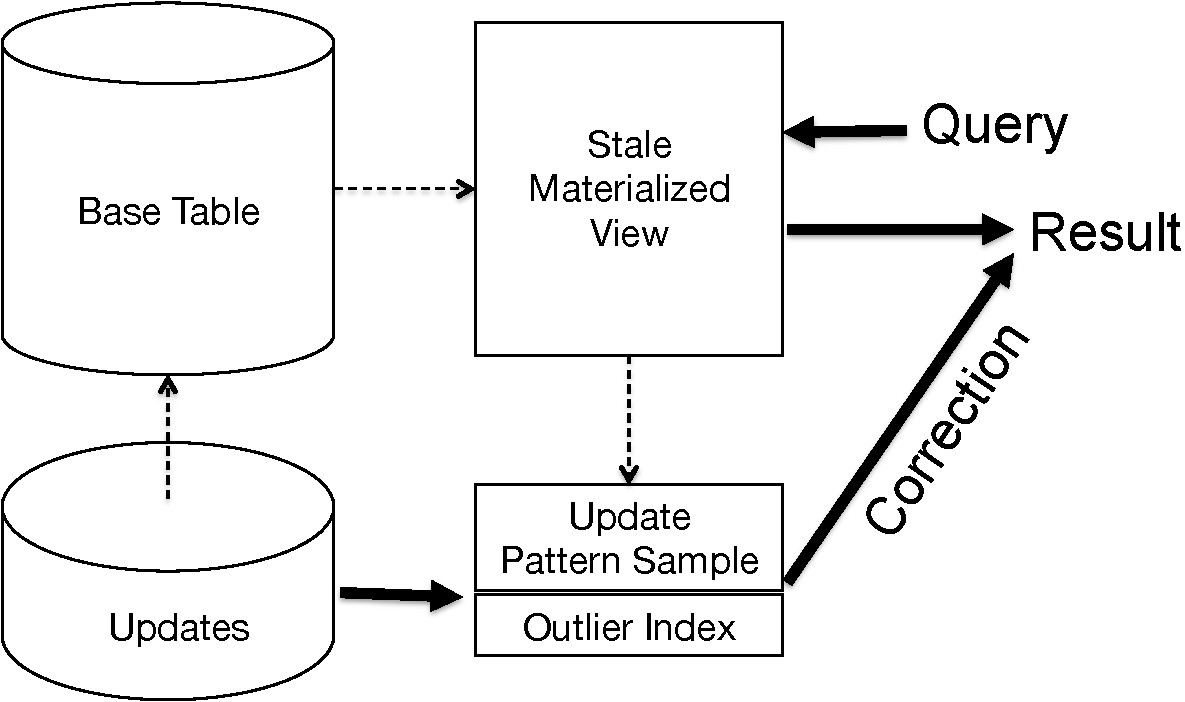
\includegraphics[scale=0.30]{figs/sys-arch.pdf}
 \caption{SVC has three main components: (1) sampling, (2) correction, and (3) outlier indexing. From a sample of up-to-date data, we estimate
 a correction for queries on stale materialized views. To make this process robust to outliers, we apply a technique called outlier indexing. \label{sys-arch}}\vspace{-1.5em}
\end{figure}

As a materialized view becomes more stale, queries on the view become increasingly inaccurate.
This closely mirrors the problem of dirty data where data errors can reduce the accuracy of query results, and data cleaning has been proposed to mitigate such inaccuracy \cite{rahm2000data}.
In this work, we explore whether refreshing stale rows in a materialized view can be modeled as a data-cleaning problem.
We take inspiration from recent results from the SampleClean data-cleaning framework which show that instead of cleaning the entire dataset,
it suffices to clean a small sample of dirty records to greatly improve query accuracy \cite{wang1999sample}.
This data-cleaning perspective raises a new possibility for materialized views, namely, that we can return more accurate results without incurring the cost of full view maintenance.
However, staleness is different sort of data error that raises interesting new challenges in sampling, cleaning, and efficient query processing.


We propose Sample-View-Clean (SVC), a framework that uses a \emph{sample} of up-to-date data to \emph{correct} stale aggregation query results.
While approximate, the corrected query result can be bounded within confidence intervals.
This framework will be complementary to existing deferred maintenance approaches; when the materialized views are stale between maintenance cycles, we can apply SVC for approximate results for a far smaller cost than having to maintain the entire view.
SVC gives results that are fresh and the user controls a bounded approximation error with the sampling ratio.


In Figure \ref{sys-arch}, we highlight the three main components of SVC: (1) sampling, (2) correction, and (3) outlier indexing. In (1), we define an ``update pattern" which represents how an update affects the view, and we sample these patterns. (2)  From the sample, we estimate how much the updates affect the query and we use this estimate to correct the stale query result.
Finally, in (3) sampling is known to be sensitive to outliers \cite{chaudhuri2001overcoming}.
We utilize a technique called outlier indexing \cite{chaudhuri2001overcoming}, which guarantees that rows in the materialized view derived from an ``outlier" record (one that has abnormal attribute values) is contained in the sample, which can be used to increase correction accuracy.

To summarize, our contributions are as follows:

\begin{itemize}\vspace{-.45em}
\item We model the incremental maintenance problem as a data cleaning problem and staleness as a type of data error.\vspace{-.45em}
\item We define the concept of ``update patterns", a logical unit that represents how an update affects a materialized view, and show how to sample the update patterns. \vspace{-.45em}
\item Using a sample of update patterns, we can correct stale aggregation queries on materialized views with bounded accuracy.\vspace{-.45em}
\item We use an outlier index to increase the accuracy of the approach for power-law, long-tailed, and skewed distributions.\vspace{-.45em}
\item We evaluate our approach on real and synthetic datasets in both single-node and distributed environments.\vspace{-.45em}
\end{itemize}

The paper is organized in the following way. 
In Section~\ref{sec-background}, we introduce materialized views and discuss the current maintenance challenges.
Next, in Section~\ref{sec-arch}, we give a brief overview of our overall system architecture.
In Section~\ref{sampling} and~\ref{correction}, we describe the sampling and query processing of our technique.
In Section~\ref{outlier}, we describe the outlier indexing framework.
In Section~\ref{sec:ext}, we discuss how our framework extends to Select queries and deletions.
Then, in Section~\ref{exp}, we evaluate our approach.
Finally, we end with our Related Work in Section~\ref{related} and our Conclusions and Future Work in Section~\ref{conclusion}.
